\section{Simulator validity test}

% Purpose of experiments
The purpose of this experiment is to test the performance and validity of the physics engine in the simulator. In particular, the interaction forces arising from contact between the snake and obstacles are studied.

The idea is to control the snake robot to a completely stretched out configuration while obstacles are symmetrically placed in contact around its center. At the same time, the snake robot should apply a constant motor torque to the center link. The obstacles are placed in a manner that prevent the joint from getting displaced. In order to still stay stretched out, all other joints will have to apply a torque calculated by the joint PID controller.

The simulator configuration for this experiment is summarized in Table \ref{tab:exp_valid1}. The link and obstacle specific configurations can be found in \ref{sec:simsetup}.

\begin{table}[h!]
    \centering
    \begin{tabular}{|c|c|c|}
        \hline
        & \textbf{Value} & \textbf{Unit}\\
        \hline \hline
        Number of obstacles & $3$ & \\
        Number of links & $14$ & \\
        Initial joint angles & $\mathbf{0}_{13 \times 1}$ & $[rad]$ \\
        $\tau_7$ & $-2$ & $[Nm]$ \\
        $[K_p, K_i, K_d]$ & $[10, 3, 0.3]$ &\\
        \hline
    \end{tabular}
    \caption{Simulation configuration for simulator validation test}
    \label{tab:exp_valid1}
\end{table}

\begin{figure}
    \centering
    
\includegraphics[width=0.9\textwidth]{figures/experiments/exp_valid1.pdf}
    \caption{Illustration of validation test}
    \label{fig:valid1_sketch}
\end{figure}

The placement of the obstacles and snake robot is illustrated in Figure \ref{fig:valid1_sketch}. As can be observed from the figure, the two outermost obstacles will establish a counter force to the resulting force from the middle joint motor torque. The resulting joint torques from this scenario are expected to comply with the well known relationship
% Math stuff
\begin{equation}
    \tau = r\times f,
\end{equation}
where $r$ is the distance from the force origin to the joint.

Since all joints are separated with equal distances and the snake robot is completely stretched out, it is expected that the torques follow a linear relationship with respect to their placement from the center. In addition, since the obstacles are symmetrically placed around the center of the robot, it is expected that the torque values are symmetrical around the center joint as well.

\begin{figure}[h!]
    \centering
    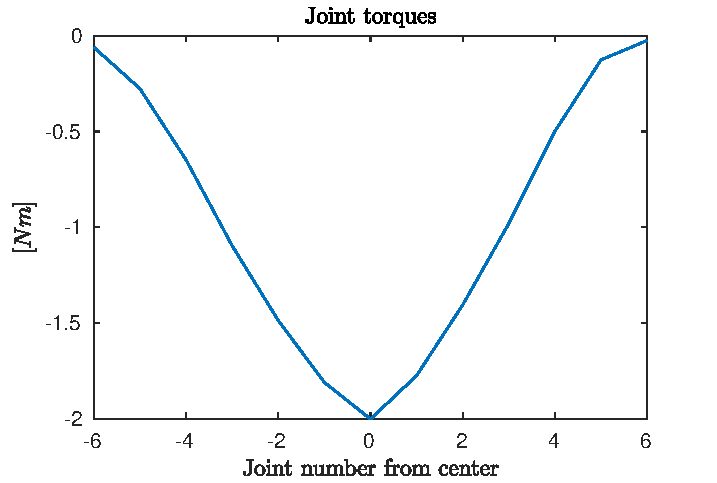
\includegraphics[width=0.9\textwidth]{figures/experiments/validation1.pdf}
    \caption{Snake robot joint torques from simulator validation test}
    \label{fig:validation1}
\end{figure}

The resulting joint torques are plotted in Figure \ref{fig:validation1}. The x-axis of this plot describes the joint number from the center joint. In order to retrieve the joint torques from the static state part of the simulation, the data was recorded after the snake robot and controller had settled into a steady state.

From the figure it is obvious that the joint torques have a close to symmetrical and linear relationship. The fifth and sixth joints from the center are exceptions here. That is however also expected since they are not between the outer and middle obstacles. A reason for why the graph is not completely linear or symmetrical is probably that it depends on the exact positioning of the obstacles and robot, and this might change slightly after the motor torques are applied. In addition, it depends to a large degree on the controllers effort to "stretch" out the snake robot. From studying Figure \ref{fig:valid1_gazebo} it is possible to see that the snake robot is ever so slightly bent.
Regardless, this experiment is considered to have validated the interaction force computations of the simulator successfully. 

\begin{figure}[h!]
    \centering
    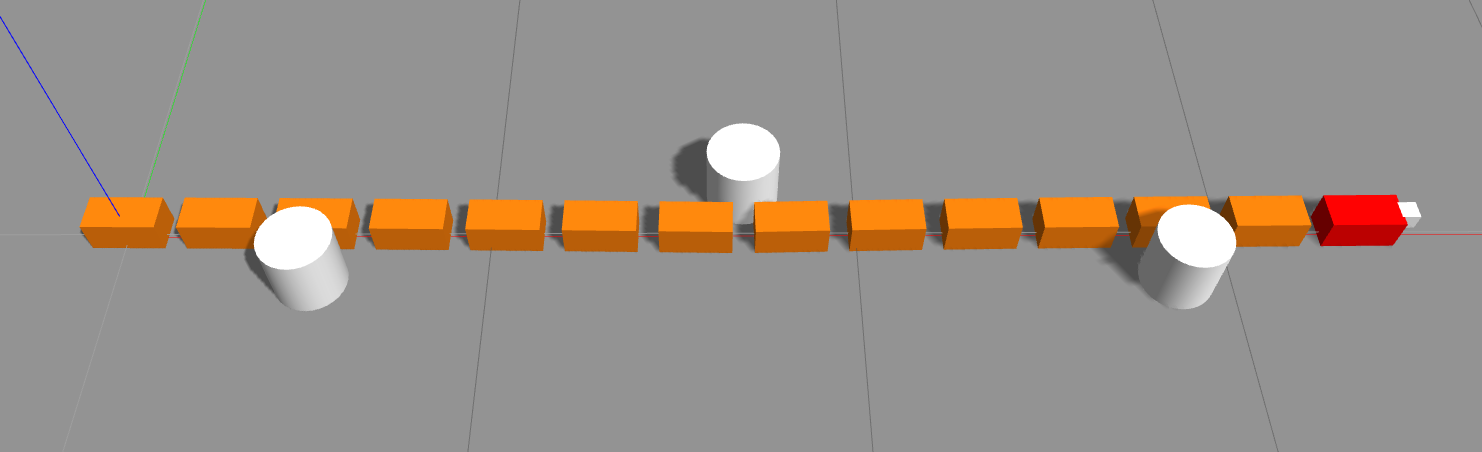
\includegraphics[width=0.9\textwidth]{figures/experiments/exp_valid1_gazebo.png}
    \caption{Screenshot from validation test Gazebo simulation}
    \label{fig:valid1_gazebo}
\end{figure}